\documentclass[]{article}

\usepackage{geometry}
\geometry{
	a4paper,
	total={170mm,257mm},
	left=20mm,
	top=20mm,
}

\usepackage[utf8]{inputenc}
\usepackage[english,russian]{babel}
\usepackage{pscyr}
\usepackage{gensymb}
\usepackage{multicol}
\usepackage{epstopdf}
\usepackage{graphicx}






\begin{document}
	
%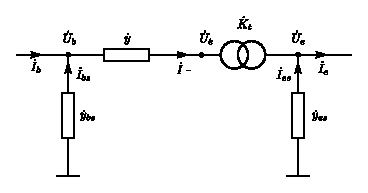
\includegraphics{piline}   

\begin {equation}
\dot{I}=(\dot{U}_e' - \dot{U}_b)\dot{y}=\left(\frac{\dot{U}_e}{\dot{K}_t}-\dot{U}_b \right) \dot{y}
\end {equation}

\begin {equation}
\dot{I}_{bs}=\dot{U}_b\dot{y}_{bs}
\end {equation}

\begin {equation}
\dot{I}_{es}=\dot{U}_e\dot{y}_{es}
\end {equation}

\begin {equation}
\dot{I}_b = \dot{I} - \dot{I}_{bs}
\end {equation}

\begin {equation}
\dot{I}_e = \frac{\dot{I}}{\hat{K}_t} + \dot{I}_{es}
\end {equation}

\begin {equation}
\dot{S}_b = \dot{U}_b\hat{I}_b
\end {equation}


\begin {equation}
\dot{S}_e = \dot{U}_e\hat{I}_e
\end {equation}


Сопряженный коэффициент по току возникает ввиду того, что:
\begin {equation}
\dot{S}_b = \dot{U}_b\hat{I}_b, \quad \dot{S}_e = \dot{U}_e\hat{I}_e, \quad \dot{S}_b=\dot{S}_e
\end {equation}

\begin {equation}
\dot{U}_e = \dot{U}_b\dot{K}_t
\end {equation}

\begin {equation}
\dot{U}_b\hat{I}_b = \dot{U}_b\dot{K}_t\hat{I}_e
\end {equation}

\begin {equation}
\dot{K}_t = \hat{\left(\frac{\dot{I}_b}{\dot{I}_e}\right)}, \quad
\hat{K}_t = {\left(\frac{\dot{I}_b}{\dot{I}_e}\right)}
\end {equation}

В матрице узловых напряжений используются собственные и взаимные проводимости:

\begin {equation}
\dot{y}_b = \frac{\dot{y}}{\dot{K}_t}
\end {equation}


\begin {equation}
\dot{y}_e = \frac{\dot{y}}{\hat{K}_t}
\end {equation}

\begin {equation}
\dot{y}_{bsa} = \dot{y}_{bs} + \dot{y}
\end {equation}

\begin {equation}
\dot{y}_{esa} = \dot{y}_{es} + \frac{\dot{y}}{K_t^2}
\end {equation}

\begin {equation}
\dot{I}_b = -\dot{y}_{bsa}\dot{U}_b + \dot{y}_b\dot{U}_e
\end {equation}

\begin {equation}
\dot{I}_e = -\dot{y}_e\dot{U}_b + \dot{y}_{esa}\dot{U}_e
\end {equation}

Так как
\begin {equation}
\dot{I}_b = -\dot{y}_{bs}\dot{U}_b - \dot{y}\dot{U}_b + \frac{\dot{y}}{\dot{K}_t}\dot{U}_e = 
-\dot{I}_{bs} + \left(\frac{\dot{U}_e}{\dot{K}_t}-\dot{U}_b\right)\dot{y}
\end {equation}

\begin {equation}
\dot{I}_e = -\frac{\dot{y}}{\hat{K_t}}\dot{U}_b + \dot{y}_{es}\dot{U}_e + \frac{\dot{y}}{K_t^2}\dot{U}_e = 
\dot{I}_{es} + \frac{1}{\hat{K}_t}\left(\frac{\dot{U}_e}{\dot{K}_t}-\dot{U}_b\right)\dot{y}
\end {equation}
\end{document}